\documentclass{scrartcl}

\usepackage[ngerman]{babel}
\usepackage[utf8]{inputenc}
\usepackage[T1]{fontenc}
\usepackage{graphicx}
\usepackage{amsmath}
\usepackage{chemmacros}
\usepackage{color}
\usepackage{enumitem}
\usepackage{icomma}
\usepackage{titlesec}
\usepackage{tikz}
\usepackage{adjustbox}
\usepackage{multirow}
\usepackage{upgreek}
\usepackage{url}
\usepackage{geometry}
 \geometry{
 a4paper,
 total={170mm,250mm},
 left=20mm,
 top=20mm,
 }

\usepackage[activate={true,nocompatibility},final]{microtype} % better font-rendering
\usepackage[bitstream-charter]{mathdesign} % bitstream font
\titleformat{\section}[hang]{
	\usefont{T1}{bch}{b}{n}\selectfont} % "bch" - Bitstream Character, "b" - bold 
	{} % label
	{0em} % horizontal separation between label and title body
	{\hspace{-0.4pt}\Large \thesection\hspace{0.6em}} % code preceding the title
	[] % additional code following the title body
\titleformat{\subsection}[hang]{
	\usefont{T1}{bch}{b}{n}\selectfont}
	{}
	{0em}
	{\hspace{-0.4pt}\large \thesubsection\hspace{0.6em}}
	[]
\titleformat{\subsubsection}[hang]{
	\usefont{T1}{bch}{b}{n}\selectfont}
	{}
	{0em}
	{\hspace{-0.4pt}\thesubsubsection\hspace{0.6em}}
	[]


\chemsetup{ modules = all }
%\usepackage[version=4]{mhchem}
\chemsetup[redox]{pos=top} % oxid. numbers on top
\usepackage{chemfig}

\newlength{\drop}

\begin{document}
  \begin{titlepage}
    \drop=0.1\textheight
    \centering
    \vspace*{\baselineskip}
    \rule{\textwidth}{1.6pt}\vspace*{-\baselineskip}\vspace*{2pt}
    \rule{\textwidth}{0.4pt}\\[\baselineskip]
    {\LARGE Versuch 1--3 (RKE)\\[0.3\baselineskip] Reaktionskinetik -- Enzyme: Aktivität und Stabilität}\\[0.2\baselineskip]
    \rule{\textwidth}{0.4pt}\vspace*{-\baselineskip}\vspace{3.2pt}
    \rule{\textwidth}{1.6pt}\\[\baselineskip]
    \scshape
    {Praktische Einführung in die Chemie\par}
    \vspace*{2\baselineskip}
    \vfill
    {\scshape Versuchstag:} \        {\large 31.05.2017}\par
  \end{titlepage}
\section{Theorieteil}
\subsection{Proteine}
Proteine sind Moleküle, die aus typischerweise zwischen 100 bis 300 \emph{Aminosäuren}, die durch \emph{Peptidbindungen} verbunden sind, bestehen. Die Funktion, die ein Protein im Organismus ausführt hängt von der \emph{Struktur} des Proteins ab. Man unterscheidet \emph{vier} verschiedene Proteinstrukturen:
\begin{enumerate}
	\item \emph{Primärstruktur:} Abfolge der einzelnen Aminosäuren in der Peptidkette.
	\item \emph{Sekundärstruktur:} Charakteristische Strukturen kürzerer Abschnitte des Proteins. Man unterscheidet z.B. zwischen $\alpha$-Helix und $\beta$-Faltblatt.
	\item \emph{Tertiärstruktur:} Räumliche Anordung des gesamten Proteins.
	\item \emph{Quartärstruktur:} Anlagerung mehrerer Proteine zu einem Komplex.
\end{enumerate}
Die meisten Proteine sind \emph{labil}, d.h. dass unter Einfluss bestimmter Umstände, wie z.B. einer \ch{pH}-Wertänderung, mechanischer Kräfte, Erwärmen und Erkalten, sie ihre \emph{Nativstruktur} und damit ihrere biologische Funktionalität verlieren. 
\subsection{Enzyme}
Enzyme sind in der Regel solche Proteine, die als \emph{Biokatalysatoren} in einem Organismus fungieren. Sie sind dafür verantwortlich biochemische Reaktionen zu beschleunigen oder gar erst zu ermöglichen. Neben der Peptidkette enhalten Enyzme sogenannte \emph{Cofaktoren}, die nicht aus Aminosäuren bestehen, für die katalytische Eigenschaft unabdingbar sind. Ist der Cofaktor \emph{fest} an dem Enzym gebunden, spricht man von der \emph{prosthetische Gruppe}, während man unter \emph{Coenzymen} solche mit \emph{transient gebundenen} (d.h. nicht fest) Cofaktoren versteht.
\subsection{Lactatdehydrogenase}
Ein wichtiges Enzym bei der \emph{anaeroben Glykolyse}, sprich Energiegewinnung der Zelle, ist die \emph{Lactatdehydrogenase} (LDH). Es katalysiert die Bildung von Lactat und \ch{NAD+} aus Pyruvat und NADH. Dies ist entscheidend in der Oxidation von Glycerinaldehyd-3-phosphat zu Glycerinaldehyd-3-phosphat-Dehydrogenase, bei der als Reduktionsäquivalent \ch{NAD+} zu NADH reduziert wird. Damit genug \ch{NAD+} vorhanden ist, dass diese Redoxreaktion stattfinden kann, wird dieses NADH mit Hilfe der LDH wieder zu \ch{NAD+} oxidiert. Das entstehende Lactat lässt sich nach intensiver Belastung der Muskulatur durch den Milchsäurespiegel nachweisen, bzw. messen. 
\subsection{Reaktionskinetik}
Die \emph{Reaktionskinetik} beschäftigt sich mit dem zeitlichen Ablauf einer Reaktion. Die grundlegende Größe ist die \emph{Reaktionsgeschwindigkeit}, die angibt, wieviele Teilchen pro Zeiteinheit in der chemischen Reaktion umgesetzt werden, was auch als \emph{Konzentrationsänderung} bezeichnet werden kann. Bei der Reaktion
\begin{equation}\label{eq:ABCD}
	a\text{ A} + b\text{ B} \ch{<=>} c\text{ C} + d\text{ D}
\end{equation}
ändern sich die Konzentrationen der Edukte und die der Produkte während der Reaktion. Läuft die Reaktion von links nach rechts, so nehmen die Konzentrationen von A und B fortwährend ab, während die der Stoffe C und D zunehmen. Die Rückreaktion verläuft analog.  

Die Reationsrate $r$ ist als die zeitliche Änderung der Konzentration definiert, für Reaktion \ref{eq:ABCD} also:
\begin{equation}
	-\frac{1}{a}\cdot\frac{dc_{\text{A}}}{dt} = -\frac{1}{b}\cdot\frac{dc_{\text{B}}}{dt} = \frac{1}{c}\cdot\frac{dc_{\text{C}}}{dt} = \frac{1}{d}\cdot\frac{dc_{\text{D}}}{dt}
\end{equation}
Im nachfolgenden Versuch wird der Reaktionsverlauf der Reaktion
\begin{equation}
	\text{Pyruvat} + \text{NADH} + \ch{H+ <=> } \text{Lactat} + \ch{NAD+}
\end{equation}
betrachtet. Dazu wird mittels eines Phonometers die Oxidation von NADH zu \ch{NAD+} betrachtet. Die Änderung der Konzentrations kann nämlich über die \emph{Extinktion} ermittelt werden, die über das \texttt{Lambert-Beersche} Gesetz wie folgt gegeben ist:
\begin{equation}\label{eq:lam}
	E = -\log{\frac{I_1}{I_0}} = \epsilon\cdot d\cdot c
\end{equation}
Wobei $I_0$ die Intensität der einfallenden Lichts, $I_1$ die des austretenden, $epsilon$ der Extinktionskoeffizient, $d$ die Dicke der Probe und $c$ die Konzentration des Stoffes ist. Durch die \emph{Änderungsrate} von $E$ lässt sich die Geschwindigkeit $v$ der Umwandlung von NADH zu \ch{NAD+} berechnen. Die Konzentration $c$ ist nach \ref{eq:lam} gegeben als:
\begin{subequations}
	\begin{align}
	c &= \frac{E}{\epsilon\cdot d} 
	\end{align}
	Woraus für $v=\frac{dc}{dt}$
	\begin{align}
		v = \frac{\Delta c}{\Delta t} &= \frac{\Delta E}{\Delta t\cdot\epsilon\cdot d} = A_V
	\end{align}
	folgt, mit $A_V$ als der \emph{Volumenaktivität}.
\end{subequations}
Da mit verdünnten Lösungen gearbeitet wird und die Volumenaktivität des Enzyms von Interesse ist, muss die Verdünnung berücksichtigt werden:
\begin{equation}
	A_V = \frac{\Delta E}{\Delta t\cdot\epsilon\cdot d}\cdot\frac{V_T}{V_P}
\end{equation}
Mit $V_P$ als dem Testvolumen und $V_P$ dem Probevolumen entspricht der Quotient dem \emph{Verdünnungsfaktor}.

 
\section{Versuche}
\subsection{Bestimmung der Reaktionsgeschwindigkeit der Reduktion von Pyruvat zu Lactat in Abhängigkeit der Konzentration aktiver LDH}
\subsubsection{Aufgabenstellung}
Der Versuch sollte die Auswirkung thermischer Zersetzung von LHD auf die Fähigkeit Pyruvat zu Lactat zu reduzieren.
\subsubsection{Versuchsdurchführung}
Zunächst wurde die Lösung ohne LDH-Lösung vorbereitet. Es wurden 9800 $\upmu$l anstatt von 980 $\upmu$l hergestellt. Dazu wurden zunächst 200 $\upmu$l NADH-Lösung mit einer Konzentration von 11 $\frac{\text{mg}}{\text{ml}}$ hinzugegeben. Nachfolgend 200 $\upmu$l Pyruvatlösung mit einer Konzentration von 2.75 $\frac{\text{mg}}{\text{ml}}$. Zuletzt werden 9,4 ml eines 67 mM Phosphatpuffers (\ch{pH} 7,2) hinzugegeben.

Nun wurde die LDH-Lösung vorbereitet. Dazu wurde LDH aus einem Schweineherzmuskel so verdünnt, dass es eine Volumenaktivität von 2-4 $\frac{\text{U}}{\text{ml}}$ aufweist. In 9 seperate Eppendorf-Reaktionsgefäße wurden nun jeweils 20 $\upmu$l der Lösung gegeben. Diese wurden nun unterschiedlich Lange in einem Thermoblock erhitzt: 0,2,5,8,12,16,20,25,30 Minuten.

Nach dem Erhitzen wurden sie zu jeweils 980 $\upmu$l der vorher hergestellten Lösung in eine Küvette gegeben, gut durchmischt und die Restaktivität bestimmt. Dies wurde mithilfe eines Spektrometers und eines Schreibers durchgeführt. Das Spektrometer musste dazu im abs- und rate-Modus eingestellt sein. Jedes mal wenn der Schreiber eine gewisse aber konstante Höhe (bei uns 6 cm) erreichte, wurde die Messung beendet und die Gerade vermessen.
\subsubsection{Beobachtung}
Wir erhielten aufgrund einer Fehlfunktion des Gerätes fremde Messwerte. Zudem waren dies nur 5 anstatt von 9.
Wir erhielten folgende Steigungen auf dem Blatt des Schreibers.
\begin{enumerate}
	\item $\frac{32 ~\text{mm}}{34\text{ mm}}$
	\item $\frac{12\text{ mm}}{19\text{ mm}}$
	\item $\frac{\hfill 4\text{ mm}}{10\text{ mm}}$
	\item $\frac{\hfill 4\text{ mm}}{10 \text{ mm}}$
	\item $\frac{\hfill 7\text{ mm}}{20\text{ mm}}$
\end{enumerate}
\subsubsection{Auswertung}
Die Enzymaktivität lässt sich mit folgender Formel berechnen:
\begin{equation}
	A_{v}=\frac{\Delta E}{\Delta t \epsilon d}\cdot \frac{V_{r}}{V_{\text{p}}}
\end{equation}
Hierbei ist $\Delta E$ die Änderung des Extinktionsfaktors, $\Delta t$ die verstrichene Zeit in Minuten, $\epsilon$ der Extinktionskoeffizient, $d$ die Strecke die das Licht durch die Probelösung zurücklegt, $V_{r}$ das Testvolument und $V_{p}$ das Probevolumen.
In unserem Fall sind dies $\epsilon=\frac{3,3 \text{ ml}}{\upmu\text{mol}\cdot\text{cm}}$, $d=1$ cm, $V_{r}=1000\;\upmu\text{l}$ und $V_{p}=20\;\upmu\text{l}$.

$\Delta E$ ergibt sich aus der y-Strecke (Zahl über dem Bruchstrich) geteilt durch 200 mm pro $\Delta E$. (Einstellung des Schreibers)
Setzt man nun die 5 Messwerte in die oben genannte Gleichung ein, so erhält man für die Küvetten die folgenden 5 Enzymaktivitäten:

\begin{figure}[h]
	\centering
	\caption{Berechnung der $\Delta E$, $\Delta t$ und $A_v$}
\begin{tabular}{c r r}
	$\Delta E$ & $\Delta t$ in min & $A_v$ in $\frac{\upmu\text{mol}}{\text{min}\cdot\text{ml}}$ \\ \hline
   	0.16 & 0.566 &4.2781 \\
     	0.06 & 0.316 &2.8708 \\
    	0.02 & 0.166 &1.8182 \\ 
     	0.02 & 0.166 & 1.8182 \\
      	0.035 & 0.333 &1.5909
\end{tabular}
\end{figure}
\begin{figure}
	\centering
	\caption{Messwerte über lineare Skala mit exponentiellem Curve fit}
	% GNUPLOT: LaTeX picture
\setlength{\unitlength}{0.240900pt}
\ifx\plotpoint\undefined\newsavebox{\plotpoint}\fi
\sbox{\plotpoint}{\rule[-0.200pt]{0.400pt}{0.400pt}}%
\begin{picture}(1500,900)(0,0)
\sbox{\plotpoint}{\rule[-0.200pt]{0.400pt}{0.400pt}}%
\put(191.0,131.0){\rule[-0.200pt]{4.818pt}{0.400pt}}
\put(171,131){\makebox(0,0)[r]{$-7$}}
\put(1419.0,131.0){\rule[-0.200pt]{4.818pt}{0.400pt}}
\put(191.0,222.0){\rule[-0.200pt]{4.818pt}{0.400pt}}
\put(171,222){\makebox(0,0)[r]{$-6.8$}}
\put(1419.0,222.0){\rule[-0.200pt]{4.818pt}{0.400pt}}
\put(191.0,313.0){\rule[-0.200pt]{4.818pt}{0.400pt}}
\put(171,313){\makebox(0,0)[r]{$-6.6$}}
\put(1419.0,313.0){\rule[-0.200pt]{4.818pt}{0.400pt}}
\put(191.0,404.0){\rule[-0.200pt]{4.818pt}{0.400pt}}
\put(171,404){\makebox(0,0)[r]{$-6.4$}}
\put(1419.0,404.0){\rule[-0.200pt]{4.818pt}{0.400pt}}
\put(191.0,495.0){\rule[-0.200pt]{4.818pt}{0.400pt}}
\put(171,495){\makebox(0,0)[r]{$-6.2$}}
\put(1419.0,495.0){\rule[-0.200pt]{4.818pt}{0.400pt}}
\put(191.0,586.0){\rule[-0.200pt]{4.818pt}{0.400pt}}
\put(171,586){\makebox(0,0)[r]{$-6$}}
\put(1419.0,586.0){\rule[-0.200pt]{4.818pt}{0.400pt}}
\put(191.0,677.0){\rule[-0.200pt]{4.818pt}{0.400pt}}
\put(171,677){\makebox(0,0)[r]{$-5.8$}}
\put(1419.0,677.0){\rule[-0.200pt]{4.818pt}{0.400pt}}
\put(191.0,768.0){\rule[-0.200pt]{4.818pt}{0.400pt}}
\put(171,768){\makebox(0,0)[r]{$-5.6$}}
\put(1419.0,768.0){\rule[-0.200pt]{4.818pt}{0.400pt}}
\put(191.0,859.0){\rule[-0.200pt]{4.818pt}{0.400pt}}
\put(171,859){\makebox(0,0)[r]{$-5.4$}}
\put(1419.0,859.0){\rule[-0.200pt]{4.818pt}{0.400pt}}
\put(191.0,131.0){\rule[-0.200pt]{0.400pt}{4.818pt}}
\put(191,90){\makebox(0,0){$0.001$}}
\put(191.0,839.0){\rule[-0.200pt]{0.400pt}{4.818pt}}
\put(399.0,131.0){\rule[-0.200pt]{0.400pt}{4.818pt}}
\put(399,90){\makebox(0,0){$0.00105$}}
\put(399.0,839.0){\rule[-0.200pt]{0.400pt}{4.818pt}}
\put(607.0,131.0){\rule[-0.200pt]{0.400pt}{4.818pt}}
\put(607,90){\makebox(0,0){$0.0011$}}
\put(607.0,839.0){\rule[-0.200pt]{0.400pt}{4.818pt}}
\put(815.0,131.0){\rule[-0.200pt]{0.400pt}{4.818pt}}
\put(815,90){\makebox(0,0){$0.00115$}}
\put(815.0,839.0){\rule[-0.200pt]{0.400pt}{4.818pt}}
\put(1023.0,131.0){\rule[-0.200pt]{0.400pt}{4.818pt}}
\put(1023,90){\makebox(0,0){$0.0012$}}
\put(1023.0,839.0){\rule[-0.200pt]{0.400pt}{4.818pt}}
\put(1231.0,131.0){\rule[-0.200pt]{0.400pt}{4.818pt}}
\put(1231,90){\makebox(0,0){$0.00125$}}
\put(1231.0,839.0){\rule[-0.200pt]{0.400pt}{4.818pt}}
\put(1439.0,131.0){\rule[-0.200pt]{0.400pt}{4.818pt}}
\put(1439,90){\makebox(0,0){$0.0013$}}
\put(1439.0,839.0){\rule[-0.200pt]{0.400pt}{4.818pt}}
\put(191.0,131.0){\rule[-0.200pt]{0.400pt}{175.375pt}}
\put(191.0,131.0){\rule[-0.200pt]{300.643pt}{0.400pt}}
\put(1439.0,131.0){\rule[-0.200pt]{0.400pt}{175.375pt}}
\put(191.0,859.0){\rule[-0.200pt]{300.643pt}{0.400pt}}
\put(30,495){\makebox(0,0){ln K}}
\put(815,29){\makebox(0,0){1/T}}
\put(1279,818){\makebox(0,0)[r]{K gemittelt}}
\put(1412,771){\makebox(0,0){$+$}}
\put(965,605){\makebox(0,0){$+$}}
\put(587,362){\makebox(0,0){$+$}}
\put(306,138){\makebox(0,0){$+$}}
\put(1349,818){\makebox(0,0){$+$}}
\put(1279,777){\makebox(0,0)[r]{y = 5219.6804*x -12.2624}}
\put(1299.0,777.0){\rule[-0.200pt]{24.090pt}{0.400pt}}
\put(306,177){\usebox{\plotpoint}}
\multiput(306.00,177.59)(0.943,0.482){9}{\rule{0.833pt}{0.116pt}}
\multiput(306.00,176.17)(9.270,6.000){2}{\rule{0.417pt}{0.400pt}}
\multiput(317.00,183.59)(0.798,0.485){11}{\rule{0.729pt}{0.117pt}}
\multiput(317.00,182.17)(9.488,7.000){2}{\rule{0.364pt}{0.400pt}}
\multiput(328.00,190.59)(0.943,0.482){9}{\rule{0.833pt}{0.116pt}}
\multiput(328.00,189.17)(9.270,6.000){2}{\rule{0.417pt}{0.400pt}}
\multiput(339.00,196.59)(0.798,0.485){11}{\rule{0.729pt}{0.117pt}}
\multiput(339.00,195.17)(9.488,7.000){2}{\rule{0.364pt}{0.400pt}}
\multiput(350.00,203.59)(1.033,0.482){9}{\rule{0.900pt}{0.116pt}}
\multiput(350.00,202.17)(10.132,6.000){2}{\rule{0.450pt}{0.400pt}}
\multiput(362.00,209.59)(0.943,0.482){9}{\rule{0.833pt}{0.116pt}}
\multiput(362.00,208.17)(9.270,6.000){2}{\rule{0.417pt}{0.400pt}}
\multiput(373.00,215.59)(0.798,0.485){11}{\rule{0.729pt}{0.117pt}}
\multiput(373.00,214.17)(9.488,7.000){2}{\rule{0.364pt}{0.400pt}}
\multiput(384.00,222.59)(0.943,0.482){9}{\rule{0.833pt}{0.116pt}}
\multiput(384.00,221.17)(9.270,6.000){2}{\rule{0.417pt}{0.400pt}}
\multiput(395.00,228.59)(0.943,0.482){9}{\rule{0.833pt}{0.116pt}}
\multiput(395.00,227.17)(9.270,6.000){2}{\rule{0.417pt}{0.400pt}}
\multiput(406.00,234.59)(0.798,0.485){11}{\rule{0.729pt}{0.117pt}}
\multiput(406.00,233.17)(9.488,7.000){2}{\rule{0.364pt}{0.400pt}}
\multiput(417.00,241.59)(1.033,0.482){9}{\rule{0.900pt}{0.116pt}}
\multiput(417.00,240.17)(10.132,6.000){2}{\rule{0.450pt}{0.400pt}}
\multiput(429.00,247.59)(0.798,0.485){11}{\rule{0.729pt}{0.117pt}}
\multiput(429.00,246.17)(9.488,7.000){2}{\rule{0.364pt}{0.400pt}}
\multiput(440.00,254.59)(0.943,0.482){9}{\rule{0.833pt}{0.116pt}}
\multiput(440.00,253.17)(9.270,6.000){2}{\rule{0.417pt}{0.400pt}}
\multiput(451.00,260.59)(0.943,0.482){9}{\rule{0.833pt}{0.116pt}}
\multiput(451.00,259.17)(9.270,6.000){2}{\rule{0.417pt}{0.400pt}}
\multiput(462.00,266.59)(0.798,0.485){11}{\rule{0.729pt}{0.117pt}}
\multiput(462.00,265.17)(9.488,7.000){2}{\rule{0.364pt}{0.400pt}}
\multiput(473.00,273.59)(0.943,0.482){9}{\rule{0.833pt}{0.116pt}}
\multiput(473.00,272.17)(9.270,6.000){2}{\rule{0.417pt}{0.400pt}}
\multiput(484.00,279.59)(1.033,0.482){9}{\rule{0.900pt}{0.116pt}}
\multiput(484.00,278.17)(10.132,6.000){2}{\rule{0.450pt}{0.400pt}}
\multiput(496.00,285.59)(0.798,0.485){11}{\rule{0.729pt}{0.117pt}}
\multiput(496.00,284.17)(9.488,7.000){2}{\rule{0.364pt}{0.400pt}}
\multiput(507.00,292.59)(0.943,0.482){9}{\rule{0.833pt}{0.116pt}}
\multiput(507.00,291.17)(9.270,6.000){2}{\rule{0.417pt}{0.400pt}}
\multiput(518.00,298.59)(0.798,0.485){11}{\rule{0.729pt}{0.117pt}}
\multiput(518.00,297.17)(9.488,7.000){2}{\rule{0.364pt}{0.400pt}}
\multiput(529.00,305.59)(0.943,0.482){9}{\rule{0.833pt}{0.116pt}}
\multiput(529.00,304.17)(9.270,6.000){2}{\rule{0.417pt}{0.400pt}}
\multiput(540.00,311.59)(1.033,0.482){9}{\rule{0.900pt}{0.116pt}}
\multiput(540.00,310.17)(10.132,6.000){2}{\rule{0.450pt}{0.400pt}}
\multiput(552.00,317.59)(0.798,0.485){11}{\rule{0.729pt}{0.117pt}}
\multiput(552.00,316.17)(9.488,7.000){2}{\rule{0.364pt}{0.400pt}}
\multiput(563.00,324.59)(0.943,0.482){9}{\rule{0.833pt}{0.116pt}}
\multiput(563.00,323.17)(9.270,6.000){2}{\rule{0.417pt}{0.400pt}}
\multiput(574.00,330.59)(0.943,0.482){9}{\rule{0.833pt}{0.116pt}}
\multiput(574.00,329.17)(9.270,6.000){2}{\rule{0.417pt}{0.400pt}}
\multiput(585.00,336.59)(0.798,0.485){11}{\rule{0.729pt}{0.117pt}}
\multiput(585.00,335.17)(9.488,7.000){2}{\rule{0.364pt}{0.400pt}}
\multiput(596.00,343.59)(0.943,0.482){9}{\rule{0.833pt}{0.116pt}}
\multiput(596.00,342.17)(9.270,6.000){2}{\rule{0.417pt}{0.400pt}}
\multiput(607.00,349.59)(0.874,0.485){11}{\rule{0.786pt}{0.117pt}}
\multiput(607.00,348.17)(10.369,7.000){2}{\rule{0.393pt}{0.400pt}}
\multiput(619.00,356.59)(0.943,0.482){9}{\rule{0.833pt}{0.116pt}}
\multiput(619.00,355.17)(9.270,6.000){2}{\rule{0.417pt}{0.400pt}}
\multiput(630.00,362.59)(0.943,0.482){9}{\rule{0.833pt}{0.116pt}}
\multiput(630.00,361.17)(9.270,6.000){2}{\rule{0.417pt}{0.400pt}}
\multiput(641.00,368.59)(0.798,0.485){11}{\rule{0.729pt}{0.117pt}}
\multiput(641.00,367.17)(9.488,7.000){2}{\rule{0.364pt}{0.400pt}}
\multiput(652.00,375.59)(0.943,0.482){9}{\rule{0.833pt}{0.116pt}}
\multiput(652.00,374.17)(9.270,6.000){2}{\rule{0.417pt}{0.400pt}}
\multiput(663.00,381.59)(0.798,0.485){11}{\rule{0.729pt}{0.117pt}}
\multiput(663.00,380.17)(9.488,7.000){2}{\rule{0.364pt}{0.400pt}}
\multiput(674.00,388.59)(1.033,0.482){9}{\rule{0.900pt}{0.116pt}}
\multiput(674.00,387.17)(10.132,6.000){2}{\rule{0.450pt}{0.400pt}}
\multiput(686.00,394.59)(0.943,0.482){9}{\rule{0.833pt}{0.116pt}}
\multiput(686.00,393.17)(9.270,6.000){2}{\rule{0.417pt}{0.400pt}}
\multiput(697.00,400.59)(0.798,0.485){11}{\rule{0.729pt}{0.117pt}}
\multiput(697.00,399.17)(9.488,7.000){2}{\rule{0.364pt}{0.400pt}}
\multiput(708.00,407.59)(0.943,0.482){9}{\rule{0.833pt}{0.116pt}}
\multiput(708.00,406.17)(9.270,6.000){2}{\rule{0.417pt}{0.400pt}}
\multiput(719.00,413.59)(0.943,0.482){9}{\rule{0.833pt}{0.116pt}}
\multiput(719.00,412.17)(9.270,6.000){2}{\rule{0.417pt}{0.400pt}}
\multiput(730.00,419.59)(0.798,0.485){11}{\rule{0.729pt}{0.117pt}}
\multiput(730.00,418.17)(9.488,7.000){2}{\rule{0.364pt}{0.400pt}}
\multiput(741.00,426.59)(1.033,0.482){9}{\rule{0.900pt}{0.116pt}}
\multiput(741.00,425.17)(10.132,6.000){2}{\rule{0.450pt}{0.400pt}}
\multiput(753.00,432.59)(0.798,0.485){11}{\rule{0.729pt}{0.117pt}}
\multiput(753.00,431.17)(9.488,7.000){2}{\rule{0.364pt}{0.400pt}}
\multiput(764.00,439.59)(0.943,0.482){9}{\rule{0.833pt}{0.116pt}}
\multiput(764.00,438.17)(9.270,6.000){2}{\rule{0.417pt}{0.400pt}}
\multiput(775.00,445.59)(0.943,0.482){9}{\rule{0.833pt}{0.116pt}}
\multiput(775.00,444.17)(9.270,6.000){2}{\rule{0.417pt}{0.400pt}}
\multiput(786.00,451.59)(0.798,0.485){11}{\rule{0.729pt}{0.117pt}}
\multiput(786.00,450.17)(9.488,7.000){2}{\rule{0.364pt}{0.400pt}}
\multiput(797.00,458.59)(0.943,0.482){9}{\rule{0.833pt}{0.116pt}}
\multiput(797.00,457.17)(9.270,6.000){2}{\rule{0.417pt}{0.400pt}}
\multiput(808.00,464.59)(1.033,0.482){9}{\rule{0.900pt}{0.116pt}}
\multiput(808.00,463.17)(10.132,6.000){2}{\rule{0.450pt}{0.400pt}}
\multiput(820.00,470.59)(0.798,0.485){11}{\rule{0.729pt}{0.117pt}}
\multiput(820.00,469.17)(9.488,7.000){2}{\rule{0.364pt}{0.400pt}}
\multiput(831.00,477.59)(0.943,0.482){9}{\rule{0.833pt}{0.116pt}}
\multiput(831.00,476.17)(9.270,6.000){2}{\rule{0.417pt}{0.400pt}}
\multiput(842.00,483.59)(0.798,0.485){11}{\rule{0.729pt}{0.117pt}}
\multiput(842.00,482.17)(9.488,7.000){2}{\rule{0.364pt}{0.400pt}}
\multiput(853.00,490.59)(0.943,0.482){9}{\rule{0.833pt}{0.116pt}}
\multiput(853.00,489.17)(9.270,6.000){2}{\rule{0.417pt}{0.400pt}}
\multiput(864.00,496.59)(0.943,0.482){9}{\rule{0.833pt}{0.116pt}}
\multiput(864.00,495.17)(9.270,6.000){2}{\rule{0.417pt}{0.400pt}}
\multiput(875.00,502.59)(0.874,0.485){11}{\rule{0.786pt}{0.117pt}}
\multiput(875.00,501.17)(10.369,7.000){2}{\rule{0.393pt}{0.400pt}}
\multiput(887.00,509.59)(0.943,0.482){9}{\rule{0.833pt}{0.116pt}}
\multiput(887.00,508.17)(9.270,6.000){2}{\rule{0.417pt}{0.400pt}}
\multiput(898.00,515.59)(0.943,0.482){9}{\rule{0.833pt}{0.116pt}}
\multiput(898.00,514.17)(9.270,6.000){2}{\rule{0.417pt}{0.400pt}}
\multiput(909.00,521.59)(0.798,0.485){11}{\rule{0.729pt}{0.117pt}}
\multiput(909.00,520.17)(9.488,7.000){2}{\rule{0.364pt}{0.400pt}}
\multiput(920.00,528.59)(0.943,0.482){9}{\rule{0.833pt}{0.116pt}}
\multiput(920.00,527.17)(9.270,6.000){2}{\rule{0.417pt}{0.400pt}}
\multiput(931.00,534.59)(0.798,0.485){11}{\rule{0.729pt}{0.117pt}}
\multiput(931.00,533.17)(9.488,7.000){2}{\rule{0.364pt}{0.400pt}}
\multiput(942.00,541.59)(1.033,0.482){9}{\rule{0.900pt}{0.116pt}}
\multiput(942.00,540.17)(10.132,6.000){2}{\rule{0.450pt}{0.400pt}}
\multiput(954.00,547.59)(0.943,0.482){9}{\rule{0.833pt}{0.116pt}}
\multiput(954.00,546.17)(9.270,6.000){2}{\rule{0.417pt}{0.400pt}}
\multiput(965.00,553.59)(0.798,0.485){11}{\rule{0.729pt}{0.117pt}}
\multiput(965.00,552.17)(9.488,7.000){2}{\rule{0.364pt}{0.400pt}}
\multiput(976.00,560.59)(0.943,0.482){9}{\rule{0.833pt}{0.116pt}}
\multiput(976.00,559.17)(9.270,6.000){2}{\rule{0.417pt}{0.400pt}}
\multiput(987.00,566.59)(0.943,0.482){9}{\rule{0.833pt}{0.116pt}}
\multiput(987.00,565.17)(9.270,6.000){2}{\rule{0.417pt}{0.400pt}}
\multiput(998.00,572.59)(0.798,0.485){11}{\rule{0.729pt}{0.117pt}}
\multiput(998.00,571.17)(9.488,7.000){2}{\rule{0.364pt}{0.400pt}}
\multiput(1009.00,579.59)(1.033,0.482){9}{\rule{0.900pt}{0.116pt}}
\multiput(1009.00,578.17)(10.132,6.000){2}{\rule{0.450pt}{0.400pt}}
\multiput(1021.00,585.59)(0.798,0.485){11}{\rule{0.729pt}{0.117pt}}
\multiput(1021.00,584.17)(9.488,7.000){2}{\rule{0.364pt}{0.400pt}}
\multiput(1032.00,592.59)(0.943,0.482){9}{\rule{0.833pt}{0.116pt}}
\multiput(1032.00,591.17)(9.270,6.000){2}{\rule{0.417pt}{0.400pt}}
\multiput(1043.00,598.59)(0.943,0.482){9}{\rule{0.833pt}{0.116pt}}
\multiput(1043.00,597.17)(9.270,6.000){2}{\rule{0.417pt}{0.400pt}}
\multiput(1054.00,604.59)(0.798,0.485){11}{\rule{0.729pt}{0.117pt}}
\multiput(1054.00,603.17)(9.488,7.000){2}{\rule{0.364pt}{0.400pt}}
\multiput(1065.00,611.59)(0.943,0.482){9}{\rule{0.833pt}{0.116pt}}
\multiput(1065.00,610.17)(9.270,6.000){2}{\rule{0.417pt}{0.400pt}}
\multiput(1076.00,617.59)(1.033,0.482){9}{\rule{0.900pt}{0.116pt}}
\multiput(1076.00,616.17)(10.132,6.000){2}{\rule{0.450pt}{0.400pt}}
\multiput(1088.00,623.59)(0.798,0.485){11}{\rule{0.729pt}{0.117pt}}
\multiput(1088.00,622.17)(9.488,7.000){2}{\rule{0.364pt}{0.400pt}}
\multiput(1099.00,630.59)(0.943,0.482){9}{\rule{0.833pt}{0.116pt}}
\multiput(1099.00,629.17)(9.270,6.000){2}{\rule{0.417pt}{0.400pt}}
\multiput(1110.00,636.59)(0.798,0.485){11}{\rule{0.729pt}{0.117pt}}
\multiput(1110.00,635.17)(9.488,7.000){2}{\rule{0.364pt}{0.400pt}}
\multiput(1121.00,643.59)(0.943,0.482){9}{\rule{0.833pt}{0.116pt}}
\multiput(1121.00,642.17)(9.270,6.000){2}{\rule{0.417pt}{0.400pt}}
\multiput(1132.00,649.59)(1.033,0.482){9}{\rule{0.900pt}{0.116pt}}
\multiput(1132.00,648.17)(10.132,6.000){2}{\rule{0.450pt}{0.400pt}}
\multiput(1144.00,655.59)(0.798,0.485){11}{\rule{0.729pt}{0.117pt}}
\multiput(1144.00,654.17)(9.488,7.000){2}{\rule{0.364pt}{0.400pt}}
\multiput(1155.00,662.59)(0.943,0.482){9}{\rule{0.833pt}{0.116pt}}
\multiput(1155.00,661.17)(9.270,6.000){2}{\rule{0.417pt}{0.400pt}}
\multiput(1166.00,668.59)(0.943,0.482){9}{\rule{0.833pt}{0.116pt}}
\multiput(1166.00,667.17)(9.270,6.000){2}{\rule{0.417pt}{0.400pt}}
\multiput(1177.00,674.59)(0.798,0.485){11}{\rule{0.729pt}{0.117pt}}
\multiput(1177.00,673.17)(9.488,7.000){2}{\rule{0.364pt}{0.400pt}}
\multiput(1188.00,681.59)(0.943,0.482){9}{\rule{0.833pt}{0.116pt}}
\multiput(1188.00,680.17)(9.270,6.000){2}{\rule{0.417pt}{0.400pt}}
\multiput(1199.00,687.59)(0.874,0.485){11}{\rule{0.786pt}{0.117pt}}
\multiput(1199.00,686.17)(10.369,7.000){2}{\rule{0.393pt}{0.400pt}}
\multiput(1211.00,694.59)(0.943,0.482){9}{\rule{0.833pt}{0.116pt}}
\multiput(1211.00,693.17)(9.270,6.000){2}{\rule{0.417pt}{0.400pt}}
\multiput(1222.00,700.59)(0.943,0.482){9}{\rule{0.833pt}{0.116pt}}
\multiput(1222.00,699.17)(9.270,6.000){2}{\rule{0.417pt}{0.400pt}}
\multiput(1233.00,706.59)(0.798,0.485){11}{\rule{0.729pt}{0.117pt}}
\multiput(1233.00,705.17)(9.488,7.000){2}{\rule{0.364pt}{0.400pt}}
\multiput(1244.00,713.59)(0.943,0.482){9}{\rule{0.833pt}{0.116pt}}
\multiput(1244.00,712.17)(9.270,6.000){2}{\rule{0.417pt}{0.400pt}}
\multiput(1255.00,719.59)(0.943,0.482){9}{\rule{0.833pt}{0.116pt}}
\multiput(1255.00,718.17)(9.270,6.000){2}{\rule{0.417pt}{0.400pt}}
\multiput(1266.00,725.59)(0.874,0.485){11}{\rule{0.786pt}{0.117pt}}
\multiput(1266.00,724.17)(10.369,7.000){2}{\rule{0.393pt}{0.400pt}}
\multiput(1278.00,732.59)(0.943,0.482){9}{\rule{0.833pt}{0.116pt}}
\multiput(1278.00,731.17)(9.270,6.000){2}{\rule{0.417pt}{0.400pt}}
\multiput(1289.00,738.59)(0.798,0.485){11}{\rule{0.729pt}{0.117pt}}
\multiput(1289.00,737.17)(9.488,7.000){2}{\rule{0.364pt}{0.400pt}}
\multiput(1300.00,745.59)(0.943,0.482){9}{\rule{0.833pt}{0.116pt}}
\multiput(1300.00,744.17)(9.270,6.000){2}{\rule{0.417pt}{0.400pt}}
\multiput(1311.00,751.59)(0.943,0.482){9}{\rule{0.833pt}{0.116pt}}
\multiput(1311.00,750.17)(9.270,6.000){2}{\rule{0.417pt}{0.400pt}}
\multiput(1322.00,757.59)(0.798,0.485){11}{\rule{0.729pt}{0.117pt}}
\multiput(1322.00,756.17)(9.488,7.000){2}{\rule{0.364pt}{0.400pt}}
\multiput(1333.00,764.59)(1.033,0.482){9}{\rule{0.900pt}{0.116pt}}
\multiput(1333.00,763.17)(10.132,6.000){2}{\rule{0.450pt}{0.400pt}}
\multiput(1345.00,770.59)(0.798,0.485){11}{\rule{0.729pt}{0.117pt}}
\multiput(1345.00,769.17)(9.488,7.000){2}{\rule{0.364pt}{0.400pt}}
\multiput(1356.00,777.59)(0.943,0.482){9}{\rule{0.833pt}{0.116pt}}
\multiput(1356.00,776.17)(9.270,6.000){2}{\rule{0.417pt}{0.400pt}}
\multiput(1367.00,783.59)(0.943,0.482){9}{\rule{0.833pt}{0.116pt}}
\multiput(1367.00,782.17)(9.270,6.000){2}{\rule{0.417pt}{0.400pt}}
\multiput(1378.00,789.59)(0.798,0.485){11}{\rule{0.729pt}{0.117pt}}
\multiput(1378.00,788.17)(9.488,7.000){2}{\rule{0.364pt}{0.400pt}}
\multiput(1389.00,796.59)(0.943,0.482){9}{\rule{0.833pt}{0.116pt}}
\multiput(1389.00,795.17)(9.270,6.000){2}{\rule{0.417pt}{0.400pt}}
\multiput(1400.00,802.59)(1.033,0.482){9}{\rule{0.900pt}{0.116pt}}
\multiput(1400.00,801.17)(10.132,6.000){2}{\rule{0.450pt}{0.400pt}}
\put(191.0,131.0){\rule[-0.200pt]{0.400pt}{175.375pt}}
\put(191.0,131.0){\rule[-0.200pt]{300.643pt}{0.400pt}}
\put(1439.0,131.0){\rule[-0.200pt]{0.400pt}{175.375pt}}
\put(191.0,859.0){\rule[-0.200pt]{300.643pt}{0.400pt}}
\end{picture}

\end{figure}
\begin{figure}\label{fig:log}
	\centering
	\caption{Messwerte über logarithmische Skala mit linearem Curve fit}
	% GNUPLOT: LaTeX picture
\setlength{\unitlength}{0.240900pt}
\ifx\plotpoint\undefined\newsavebox{\plotpoint}\fi
\sbox{\plotpoint}{\rule[-0.200pt]{0.400pt}{0.400pt}}%
\begin{picture}(1500,900)(0,0)
\sbox{\plotpoint}{\rule[-0.200pt]{0.400pt}{0.400pt}}%
\put(191.0,131.0){\rule[-0.200pt]{4.818pt}{0.400pt}}
\put(171,131){\makebox(0,0)[r]{$0.1$}}
\put(1419.0,131.0){\rule[-0.200pt]{4.818pt}{0.400pt}}
\put(191.0,197.0){\rule[-0.200pt]{4.818pt}{0.400pt}}
\put(171,197){\makebox(0,0)[r]{$0.15$}}
\put(1419.0,197.0){\rule[-0.200pt]{4.818pt}{0.400pt}}
\put(191.0,263.0){\rule[-0.200pt]{4.818pt}{0.400pt}}
\put(171,263){\makebox(0,0)[r]{$0.2$}}
\put(1419.0,263.0){\rule[-0.200pt]{4.818pt}{0.400pt}}
\put(191.0,330.0){\rule[-0.200pt]{4.818pt}{0.400pt}}
\put(171,330){\makebox(0,0)[r]{$0.25$}}
\put(1419.0,330.0){\rule[-0.200pt]{4.818pt}{0.400pt}}
\put(191.0,396.0){\rule[-0.200pt]{4.818pt}{0.400pt}}
\put(171,396){\makebox(0,0)[r]{$0.3$}}
\put(1419.0,396.0){\rule[-0.200pt]{4.818pt}{0.400pt}}
\put(191.0,462.0){\rule[-0.200pt]{4.818pt}{0.400pt}}
\put(171,462){\makebox(0,0)[r]{$0.35$}}
\put(1419.0,462.0){\rule[-0.200pt]{4.818pt}{0.400pt}}
\put(191.0,528.0){\rule[-0.200pt]{4.818pt}{0.400pt}}
\put(171,528){\makebox(0,0)[r]{$0.4$}}
\put(1419.0,528.0){\rule[-0.200pt]{4.818pt}{0.400pt}}
\put(191.0,594.0){\rule[-0.200pt]{4.818pt}{0.400pt}}
\put(171,594){\makebox(0,0)[r]{$0.45$}}
\put(1419.0,594.0){\rule[-0.200pt]{4.818pt}{0.400pt}}
\put(191.0,660.0){\rule[-0.200pt]{4.818pt}{0.400pt}}
\put(171,660){\makebox(0,0)[r]{$0.5$}}
\put(1419.0,660.0){\rule[-0.200pt]{4.818pt}{0.400pt}}
\put(191.0,727.0){\rule[-0.200pt]{4.818pt}{0.400pt}}
\put(171,727){\makebox(0,0)[r]{$0.55$}}
\put(1419.0,727.0){\rule[-0.200pt]{4.818pt}{0.400pt}}
\put(191.0,793.0){\rule[-0.200pt]{4.818pt}{0.400pt}}
\put(171,793){\makebox(0,0)[r]{$0.6$}}
\put(1419.0,793.0){\rule[-0.200pt]{4.818pt}{0.400pt}}
\put(191.0,859.0){\rule[-0.200pt]{4.818pt}{0.400pt}}
\put(171,859){\makebox(0,0)[r]{$0.65$}}
\put(1419.0,859.0){\rule[-0.200pt]{4.818pt}{0.400pt}}
\put(191.0,131.0){\rule[-0.200pt]{0.400pt}{4.818pt}}
\put(191,90){\makebox(0,0){$0$}}
\put(191.0,839.0){\rule[-0.200pt]{0.400pt}{4.818pt}}
\put(399.0,131.0){\rule[-0.200pt]{0.400pt}{4.818pt}}
\put(399,90){\makebox(0,0){$2$}}
\put(399.0,839.0){\rule[-0.200pt]{0.400pt}{4.818pt}}
\put(607.0,131.0){\rule[-0.200pt]{0.400pt}{4.818pt}}
\put(607,90){\makebox(0,0){$4$}}
\put(607.0,839.0){\rule[-0.200pt]{0.400pt}{4.818pt}}
\put(815.0,131.0){\rule[-0.200pt]{0.400pt}{4.818pt}}
\put(815,90){\makebox(0,0){$6$}}
\put(815.0,839.0){\rule[-0.200pt]{0.400pt}{4.818pt}}
\put(1023.0,131.0){\rule[-0.200pt]{0.400pt}{4.818pt}}
\put(1023,90){\makebox(0,0){$8$}}
\put(1023.0,839.0){\rule[-0.200pt]{0.400pt}{4.818pt}}
\put(1231.0,131.0){\rule[-0.200pt]{0.400pt}{4.818pt}}
\put(1231,90){\makebox(0,0){$10$}}
\put(1231.0,839.0){\rule[-0.200pt]{0.400pt}{4.818pt}}
\put(1439.0,131.0){\rule[-0.200pt]{0.400pt}{4.818pt}}
\put(1439,90){\makebox(0,0){$12$}}
\put(1439.0,839.0){\rule[-0.200pt]{0.400pt}{4.818pt}}
\put(191.0,131.0){\rule[-0.200pt]{0.400pt}{175.375pt}}
\put(191.0,131.0){\rule[-0.200pt]{300.643pt}{0.400pt}}
\put(1439.0,131.0){\rule[-0.200pt]{0.400pt}{175.375pt}}
\put(191.0,859.0){\rule[-0.200pt]{300.643pt}{0.400pt}}
\put(30,495){\makebox(0,0){$log(A_v)$}}
\put(815,29){\makebox(0,0){t in min}}
\put(1279,818){\makebox(0,0)[r]{logarithmische Messwerte}}
\put(191,834){\makebox(0,0){$+$}}
\put(399,605){\makebox(0,0){$+$}}
\put(711,342){\makebox(0,0){$+$}}
\put(1023,342){\makebox(0,0){$+$}}
\put(1439,266){\makebox(0,0){$+$}}
\put(1349,818){\makebox(0,0){$+$}}
\put(1279,777){\makebox(0,0)[r]{f = -0.0336*t+0.5434}}
\put(1299.0,777.0){\rule[-0.200pt]{24.090pt}{0.400pt}}
\put(191,718){\usebox{\plotpoint}}
\multiput(191.00,716.93)(1.378,-0.477){7}{\rule{1.140pt}{0.115pt}}
\multiput(191.00,717.17)(10.634,-5.000){2}{\rule{0.570pt}{0.400pt}}
\multiput(204.00,711.93)(1.033,-0.482){9}{\rule{0.900pt}{0.116pt}}
\multiput(204.00,712.17)(10.132,-6.000){2}{\rule{0.450pt}{0.400pt}}
\multiput(216.00,705.93)(1.378,-0.477){7}{\rule{1.140pt}{0.115pt}}
\multiput(216.00,706.17)(10.634,-5.000){2}{\rule{0.570pt}{0.400pt}}
\multiput(229.00,700.93)(1.033,-0.482){9}{\rule{0.900pt}{0.116pt}}
\multiput(229.00,701.17)(10.132,-6.000){2}{\rule{0.450pt}{0.400pt}}
\multiput(241.00,694.93)(1.378,-0.477){7}{\rule{1.140pt}{0.115pt}}
\multiput(241.00,695.17)(10.634,-5.000){2}{\rule{0.570pt}{0.400pt}}
\multiput(254.00,689.93)(1.378,-0.477){7}{\rule{1.140pt}{0.115pt}}
\multiput(254.00,690.17)(10.634,-5.000){2}{\rule{0.570pt}{0.400pt}}
\multiput(267.00,684.93)(1.033,-0.482){9}{\rule{0.900pt}{0.116pt}}
\multiput(267.00,685.17)(10.132,-6.000){2}{\rule{0.450pt}{0.400pt}}
\multiput(279.00,678.93)(1.378,-0.477){7}{\rule{1.140pt}{0.115pt}}
\multiput(279.00,679.17)(10.634,-5.000){2}{\rule{0.570pt}{0.400pt}}
\multiput(292.00,673.93)(1.033,-0.482){9}{\rule{0.900pt}{0.116pt}}
\multiput(292.00,674.17)(10.132,-6.000){2}{\rule{0.450pt}{0.400pt}}
\multiput(304.00,667.93)(1.378,-0.477){7}{\rule{1.140pt}{0.115pt}}
\multiput(304.00,668.17)(10.634,-5.000){2}{\rule{0.570pt}{0.400pt}}
\multiput(317.00,662.93)(1.378,-0.477){7}{\rule{1.140pt}{0.115pt}}
\multiput(317.00,663.17)(10.634,-5.000){2}{\rule{0.570pt}{0.400pt}}
\multiput(330.00,657.93)(1.033,-0.482){9}{\rule{0.900pt}{0.116pt}}
\multiput(330.00,658.17)(10.132,-6.000){2}{\rule{0.450pt}{0.400pt}}
\multiput(342.00,651.93)(1.378,-0.477){7}{\rule{1.140pt}{0.115pt}}
\multiput(342.00,652.17)(10.634,-5.000){2}{\rule{0.570pt}{0.400pt}}
\multiput(355.00,646.93)(1.267,-0.477){7}{\rule{1.060pt}{0.115pt}}
\multiput(355.00,647.17)(9.800,-5.000){2}{\rule{0.530pt}{0.400pt}}
\multiput(367.00,641.93)(1.123,-0.482){9}{\rule{0.967pt}{0.116pt}}
\multiput(367.00,642.17)(10.994,-6.000){2}{\rule{0.483pt}{0.400pt}}
\multiput(380.00,635.93)(1.378,-0.477){7}{\rule{1.140pt}{0.115pt}}
\multiput(380.00,636.17)(10.634,-5.000){2}{\rule{0.570pt}{0.400pt}}
\multiput(393.00,630.93)(1.033,-0.482){9}{\rule{0.900pt}{0.116pt}}
\multiput(393.00,631.17)(10.132,-6.000){2}{\rule{0.450pt}{0.400pt}}
\multiput(405.00,624.93)(1.378,-0.477){7}{\rule{1.140pt}{0.115pt}}
\multiput(405.00,625.17)(10.634,-5.000){2}{\rule{0.570pt}{0.400pt}}
\multiput(418.00,619.93)(1.378,-0.477){7}{\rule{1.140pt}{0.115pt}}
\multiput(418.00,620.17)(10.634,-5.000){2}{\rule{0.570pt}{0.400pt}}
\multiput(431.00,614.93)(1.033,-0.482){9}{\rule{0.900pt}{0.116pt}}
\multiput(431.00,615.17)(10.132,-6.000){2}{\rule{0.450pt}{0.400pt}}
\multiput(443.00,608.93)(1.378,-0.477){7}{\rule{1.140pt}{0.115pt}}
\multiput(443.00,609.17)(10.634,-5.000){2}{\rule{0.570pt}{0.400pt}}
\multiput(456.00,603.93)(1.033,-0.482){9}{\rule{0.900pt}{0.116pt}}
\multiput(456.00,604.17)(10.132,-6.000){2}{\rule{0.450pt}{0.400pt}}
\multiput(468.00,597.93)(1.378,-0.477){7}{\rule{1.140pt}{0.115pt}}
\multiput(468.00,598.17)(10.634,-5.000){2}{\rule{0.570pt}{0.400pt}}
\multiput(481.00,592.93)(1.378,-0.477){7}{\rule{1.140pt}{0.115pt}}
\multiput(481.00,593.17)(10.634,-5.000){2}{\rule{0.570pt}{0.400pt}}
\multiput(494.00,587.93)(1.033,-0.482){9}{\rule{0.900pt}{0.116pt}}
\multiput(494.00,588.17)(10.132,-6.000){2}{\rule{0.450pt}{0.400pt}}
\multiput(506.00,581.93)(1.378,-0.477){7}{\rule{1.140pt}{0.115pt}}
\multiput(506.00,582.17)(10.634,-5.000){2}{\rule{0.570pt}{0.400pt}}
\multiput(519.00,576.93)(1.033,-0.482){9}{\rule{0.900pt}{0.116pt}}
\multiput(519.00,577.17)(10.132,-6.000){2}{\rule{0.450pt}{0.400pt}}
\multiput(531.00,570.93)(1.378,-0.477){7}{\rule{1.140pt}{0.115pt}}
\multiput(531.00,571.17)(10.634,-5.000){2}{\rule{0.570pt}{0.400pt}}
\multiput(544.00,565.93)(1.378,-0.477){7}{\rule{1.140pt}{0.115pt}}
\multiput(544.00,566.17)(10.634,-5.000){2}{\rule{0.570pt}{0.400pt}}
\multiput(557.00,560.93)(1.033,-0.482){9}{\rule{0.900pt}{0.116pt}}
\multiput(557.00,561.17)(10.132,-6.000){2}{\rule{0.450pt}{0.400pt}}
\multiput(569.00,554.93)(1.378,-0.477){7}{\rule{1.140pt}{0.115pt}}
\multiput(569.00,555.17)(10.634,-5.000){2}{\rule{0.570pt}{0.400pt}}
\multiput(582.00,549.93)(1.033,-0.482){9}{\rule{0.900pt}{0.116pt}}
\multiput(582.00,550.17)(10.132,-6.000){2}{\rule{0.450pt}{0.400pt}}
\multiput(594.00,543.93)(1.378,-0.477){7}{\rule{1.140pt}{0.115pt}}
\multiput(594.00,544.17)(10.634,-5.000){2}{\rule{0.570pt}{0.400pt}}
\multiput(607.00,538.93)(1.378,-0.477){7}{\rule{1.140pt}{0.115pt}}
\multiput(607.00,539.17)(10.634,-5.000){2}{\rule{0.570pt}{0.400pt}}
\multiput(620.00,533.93)(1.033,-0.482){9}{\rule{0.900pt}{0.116pt}}
\multiput(620.00,534.17)(10.132,-6.000){2}{\rule{0.450pt}{0.400pt}}
\multiput(632.00,527.93)(1.378,-0.477){7}{\rule{1.140pt}{0.115pt}}
\multiput(632.00,528.17)(10.634,-5.000){2}{\rule{0.570pt}{0.400pt}}
\multiput(645.00,522.93)(1.267,-0.477){7}{\rule{1.060pt}{0.115pt}}
\multiput(645.00,523.17)(9.800,-5.000){2}{\rule{0.530pt}{0.400pt}}
\multiput(657.00,517.93)(1.123,-0.482){9}{\rule{0.967pt}{0.116pt}}
\multiput(657.00,518.17)(10.994,-6.000){2}{\rule{0.483pt}{0.400pt}}
\multiput(670.00,511.93)(1.378,-0.477){7}{\rule{1.140pt}{0.115pt}}
\multiput(670.00,512.17)(10.634,-5.000){2}{\rule{0.570pt}{0.400pt}}
\multiput(683.00,506.93)(1.033,-0.482){9}{\rule{0.900pt}{0.116pt}}
\multiput(683.00,507.17)(10.132,-6.000){2}{\rule{0.450pt}{0.400pt}}
\multiput(695.00,500.93)(1.378,-0.477){7}{\rule{1.140pt}{0.115pt}}
\multiput(695.00,501.17)(10.634,-5.000){2}{\rule{0.570pt}{0.400pt}}
\multiput(708.00,495.93)(1.267,-0.477){7}{\rule{1.060pt}{0.115pt}}
\multiput(708.00,496.17)(9.800,-5.000){2}{\rule{0.530pt}{0.400pt}}
\multiput(720.00,490.93)(1.123,-0.482){9}{\rule{0.967pt}{0.116pt}}
\multiput(720.00,491.17)(10.994,-6.000){2}{\rule{0.483pt}{0.400pt}}
\multiput(733.00,484.93)(1.378,-0.477){7}{\rule{1.140pt}{0.115pt}}
\multiput(733.00,485.17)(10.634,-5.000){2}{\rule{0.570pt}{0.400pt}}
\multiput(746.00,479.93)(1.033,-0.482){9}{\rule{0.900pt}{0.116pt}}
\multiput(746.00,480.17)(10.132,-6.000){2}{\rule{0.450pt}{0.400pt}}
\multiput(758.00,473.93)(1.378,-0.477){7}{\rule{1.140pt}{0.115pt}}
\multiput(758.00,474.17)(10.634,-5.000){2}{\rule{0.570pt}{0.400pt}}
\multiput(771.00,468.93)(1.267,-0.477){7}{\rule{1.060pt}{0.115pt}}
\multiput(771.00,469.17)(9.800,-5.000){2}{\rule{0.530pt}{0.400pt}}
\multiput(783.00,463.93)(1.123,-0.482){9}{\rule{0.967pt}{0.116pt}}
\multiput(783.00,464.17)(10.994,-6.000){2}{\rule{0.483pt}{0.400pt}}
\multiput(796.00,457.93)(1.378,-0.477){7}{\rule{1.140pt}{0.115pt}}
\multiput(796.00,458.17)(10.634,-5.000){2}{\rule{0.570pt}{0.400pt}}
\multiput(809.00,452.93)(1.033,-0.482){9}{\rule{0.900pt}{0.116pt}}
\multiput(809.00,453.17)(10.132,-6.000){2}{\rule{0.450pt}{0.400pt}}
\multiput(821.00,446.93)(1.378,-0.477){7}{\rule{1.140pt}{0.115pt}}
\multiput(821.00,447.17)(10.634,-5.000){2}{\rule{0.570pt}{0.400pt}}
\multiput(834.00,441.93)(1.378,-0.477){7}{\rule{1.140pt}{0.115pt}}
\multiput(834.00,442.17)(10.634,-5.000){2}{\rule{0.570pt}{0.400pt}}
\multiput(847.00,436.93)(1.033,-0.482){9}{\rule{0.900pt}{0.116pt}}
\multiput(847.00,437.17)(10.132,-6.000){2}{\rule{0.450pt}{0.400pt}}
\multiput(859.00,430.93)(1.378,-0.477){7}{\rule{1.140pt}{0.115pt}}
\multiput(859.00,431.17)(10.634,-5.000){2}{\rule{0.570pt}{0.400pt}}
\multiput(872.00,425.93)(1.267,-0.477){7}{\rule{1.060pt}{0.115pt}}
\multiput(872.00,426.17)(9.800,-5.000){2}{\rule{0.530pt}{0.400pt}}
\multiput(884.00,420.93)(1.123,-0.482){9}{\rule{0.967pt}{0.116pt}}
\multiput(884.00,421.17)(10.994,-6.000){2}{\rule{0.483pt}{0.400pt}}
\multiput(897.00,414.93)(1.378,-0.477){7}{\rule{1.140pt}{0.115pt}}
\multiput(897.00,415.17)(10.634,-5.000){2}{\rule{0.570pt}{0.400pt}}
\multiput(910.00,409.93)(1.033,-0.482){9}{\rule{0.900pt}{0.116pt}}
\multiput(910.00,410.17)(10.132,-6.000){2}{\rule{0.450pt}{0.400pt}}
\multiput(922.00,403.93)(1.378,-0.477){7}{\rule{1.140pt}{0.115pt}}
\multiput(922.00,404.17)(10.634,-5.000){2}{\rule{0.570pt}{0.400pt}}
\multiput(935.00,398.93)(1.267,-0.477){7}{\rule{1.060pt}{0.115pt}}
\multiput(935.00,399.17)(9.800,-5.000){2}{\rule{0.530pt}{0.400pt}}
\multiput(947.00,393.93)(1.123,-0.482){9}{\rule{0.967pt}{0.116pt}}
\multiput(947.00,394.17)(10.994,-6.000){2}{\rule{0.483pt}{0.400pt}}
\multiput(960.00,387.93)(1.378,-0.477){7}{\rule{1.140pt}{0.115pt}}
\multiput(960.00,388.17)(10.634,-5.000){2}{\rule{0.570pt}{0.400pt}}
\multiput(973.00,382.93)(1.033,-0.482){9}{\rule{0.900pt}{0.116pt}}
\multiput(973.00,383.17)(10.132,-6.000){2}{\rule{0.450pt}{0.400pt}}
\multiput(985.00,376.93)(1.378,-0.477){7}{\rule{1.140pt}{0.115pt}}
\multiput(985.00,377.17)(10.634,-5.000){2}{\rule{0.570pt}{0.400pt}}
\multiput(998.00,371.93)(1.267,-0.477){7}{\rule{1.060pt}{0.115pt}}
\multiput(998.00,372.17)(9.800,-5.000){2}{\rule{0.530pt}{0.400pt}}
\multiput(1010.00,366.93)(1.123,-0.482){9}{\rule{0.967pt}{0.116pt}}
\multiput(1010.00,367.17)(10.994,-6.000){2}{\rule{0.483pt}{0.400pt}}
\multiput(1023.00,360.93)(1.378,-0.477){7}{\rule{1.140pt}{0.115pt}}
\multiput(1023.00,361.17)(10.634,-5.000){2}{\rule{0.570pt}{0.400pt}}
\multiput(1036.00,355.93)(1.033,-0.482){9}{\rule{0.900pt}{0.116pt}}
\multiput(1036.00,356.17)(10.132,-6.000){2}{\rule{0.450pt}{0.400pt}}
\multiput(1048.00,349.93)(1.378,-0.477){7}{\rule{1.140pt}{0.115pt}}
\multiput(1048.00,350.17)(10.634,-5.000){2}{\rule{0.570pt}{0.400pt}}
\multiput(1061.00,344.93)(1.267,-0.477){7}{\rule{1.060pt}{0.115pt}}
\multiput(1061.00,345.17)(9.800,-5.000){2}{\rule{0.530pt}{0.400pt}}
\multiput(1073.00,339.93)(1.123,-0.482){9}{\rule{0.967pt}{0.116pt}}
\multiput(1073.00,340.17)(10.994,-6.000){2}{\rule{0.483pt}{0.400pt}}
\multiput(1086.00,333.93)(1.378,-0.477){7}{\rule{1.140pt}{0.115pt}}
\multiput(1086.00,334.17)(10.634,-5.000){2}{\rule{0.570pt}{0.400pt}}
\multiput(1099.00,328.93)(1.033,-0.482){9}{\rule{0.900pt}{0.116pt}}
\multiput(1099.00,329.17)(10.132,-6.000){2}{\rule{0.450pt}{0.400pt}}
\multiput(1111.00,322.93)(1.378,-0.477){7}{\rule{1.140pt}{0.115pt}}
\multiput(1111.00,323.17)(10.634,-5.000){2}{\rule{0.570pt}{0.400pt}}
\multiput(1124.00,317.93)(1.267,-0.477){7}{\rule{1.060pt}{0.115pt}}
\multiput(1124.00,318.17)(9.800,-5.000){2}{\rule{0.530pt}{0.400pt}}
\multiput(1136.00,312.93)(1.123,-0.482){9}{\rule{0.967pt}{0.116pt}}
\multiput(1136.00,313.17)(10.994,-6.000){2}{\rule{0.483pt}{0.400pt}}
\multiput(1149.00,306.93)(1.378,-0.477){7}{\rule{1.140pt}{0.115pt}}
\multiput(1149.00,307.17)(10.634,-5.000){2}{\rule{0.570pt}{0.400pt}}
\multiput(1162.00,301.93)(1.267,-0.477){7}{\rule{1.060pt}{0.115pt}}
\multiput(1162.00,302.17)(9.800,-5.000){2}{\rule{0.530pt}{0.400pt}}
\multiput(1174.00,296.93)(1.123,-0.482){9}{\rule{0.967pt}{0.116pt}}
\multiput(1174.00,297.17)(10.994,-6.000){2}{\rule{0.483pt}{0.400pt}}
\multiput(1187.00,290.93)(1.267,-0.477){7}{\rule{1.060pt}{0.115pt}}
\multiput(1187.00,291.17)(9.800,-5.000){2}{\rule{0.530pt}{0.400pt}}
\multiput(1199.00,285.93)(1.123,-0.482){9}{\rule{0.967pt}{0.116pt}}
\multiput(1199.00,286.17)(10.994,-6.000){2}{\rule{0.483pt}{0.400pt}}
\multiput(1212.00,279.93)(1.378,-0.477){7}{\rule{1.140pt}{0.115pt}}
\multiput(1212.00,280.17)(10.634,-5.000){2}{\rule{0.570pt}{0.400pt}}
\multiput(1225.00,274.93)(1.267,-0.477){7}{\rule{1.060pt}{0.115pt}}
\multiput(1225.00,275.17)(9.800,-5.000){2}{\rule{0.530pt}{0.400pt}}
\multiput(1237.00,269.93)(1.123,-0.482){9}{\rule{0.967pt}{0.116pt}}
\multiput(1237.00,270.17)(10.994,-6.000){2}{\rule{0.483pt}{0.400pt}}
\multiput(1250.00,263.93)(1.378,-0.477){7}{\rule{1.140pt}{0.115pt}}
\multiput(1250.00,264.17)(10.634,-5.000){2}{\rule{0.570pt}{0.400pt}}
\multiput(1263.00,258.93)(1.033,-0.482){9}{\rule{0.900pt}{0.116pt}}
\multiput(1263.00,259.17)(10.132,-6.000){2}{\rule{0.450pt}{0.400pt}}
\multiput(1275.00,252.93)(1.378,-0.477){7}{\rule{1.140pt}{0.115pt}}
\multiput(1275.00,253.17)(10.634,-5.000){2}{\rule{0.570pt}{0.400pt}}
\multiput(1288.00,247.93)(1.267,-0.477){7}{\rule{1.060pt}{0.115pt}}
\multiput(1288.00,248.17)(9.800,-5.000){2}{\rule{0.530pt}{0.400pt}}
\multiput(1300.00,242.93)(1.123,-0.482){9}{\rule{0.967pt}{0.116pt}}
\multiput(1300.00,243.17)(10.994,-6.000){2}{\rule{0.483pt}{0.400pt}}
\multiput(1313.00,236.93)(1.378,-0.477){7}{\rule{1.140pt}{0.115pt}}
\multiput(1313.00,237.17)(10.634,-5.000){2}{\rule{0.570pt}{0.400pt}}
\multiput(1326.00,231.93)(1.033,-0.482){9}{\rule{0.900pt}{0.116pt}}
\multiput(1326.00,232.17)(10.132,-6.000){2}{\rule{0.450pt}{0.400pt}}
\multiput(1338.00,225.93)(1.378,-0.477){7}{\rule{1.140pt}{0.115pt}}
\multiput(1338.00,226.17)(10.634,-5.000){2}{\rule{0.570pt}{0.400pt}}
\multiput(1351.00,220.93)(1.267,-0.477){7}{\rule{1.060pt}{0.115pt}}
\multiput(1351.00,221.17)(9.800,-5.000){2}{\rule{0.530pt}{0.400pt}}
\multiput(1363.00,215.93)(1.123,-0.482){9}{\rule{0.967pt}{0.116pt}}
\multiput(1363.00,216.17)(10.994,-6.000){2}{\rule{0.483pt}{0.400pt}}
\multiput(1376.00,209.93)(1.378,-0.477){7}{\rule{1.140pt}{0.115pt}}
\multiput(1376.00,210.17)(10.634,-5.000){2}{\rule{0.570pt}{0.400pt}}
\multiput(1389.00,204.93)(1.267,-0.477){7}{\rule{1.060pt}{0.115pt}}
\multiput(1389.00,205.17)(9.800,-5.000){2}{\rule{0.530pt}{0.400pt}}
\multiput(1401.00,199.93)(1.123,-0.482){9}{\rule{0.967pt}{0.116pt}}
\multiput(1401.00,200.17)(10.994,-6.000){2}{\rule{0.483pt}{0.400pt}}
\multiput(1414.00,193.93)(1.267,-0.477){7}{\rule{1.060pt}{0.115pt}}
\multiput(1414.00,194.17)(9.800,-5.000){2}{\rule{0.530pt}{0.400pt}}
\multiput(1426.00,188.93)(1.123,-0.482){9}{\rule{0.967pt}{0.116pt}}
\multiput(1426.00,189.17)(10.994,-6.000){2}{\rule{0.483pt}{0.400pt}}
\put(191.0,131.0){\rule[-0.200pt]{0.400pt}{175.375pt}}
\put(191.0,131.0){\rule[-0.200pt]{300.643pt}{0.400pt}}
\put(1439.0,131.0){\rule[-0.200pt]{0.400pt}{175.375pt}}
\put(191.0,859.0){\rule[-0.200pt]{300.643pt}{0.400pt}}
\end{picture}

\end{figure}

Die eben berechneten Werte können nun in ein x-$A_{v}$ Diagramm eingetragen werden. Man kann nun mithilfe einer Exponentialfunktion eine Kurve konstruieren (Diagramm 1) oder mit einer Geraden darstellen falls man die Logarithmischen Werte nimmt (Diagramm 2)
Aus der Steigung der Gerade kann nun die Halbwertszeit hergeleitet werden:
\begin{equation}
	T_{\frac{1}{2}} = |\frac{\ln{2}}{k}| = 18.9384\text{ min}
\end{equation}
$k = -0.0336$ lässt sich aus Abbildung \ref{fig:log} auslesen.

\newpage
\subsubsection*{Reaktionsgleichung}
\begin{figure}[h]
	\centering
	\caption{Reduktion von Pyruvat zu Lactat\protect\footnotemark}
	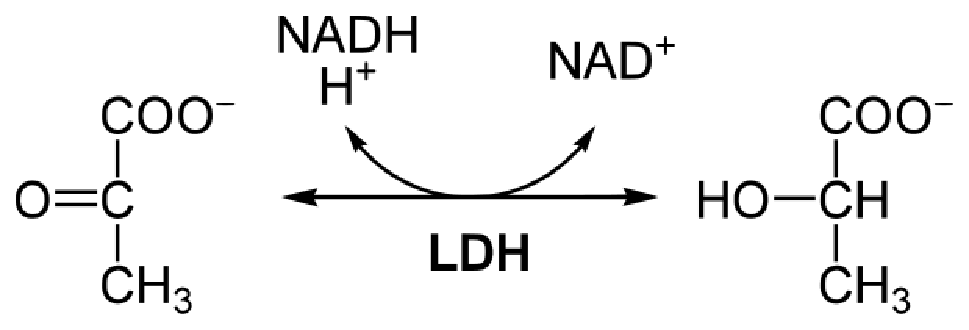
\includegraphics[scale=.5]{LDH_reaction.pdf}
	\end{figure}
	\footnotetext{\url{https://commons.wikimedia.org/wiki/File:LDH_reaction.svg#/media/File:LDH_reaction.svg}}
	\begin{figure}[h]
	\centering
	\caption{Oxidationszahlen}
	\begin{tabular}{c c}
			Linke Seite & Rechte Seite \\ \hline
			O = -2 & H = 1 \\
			C = 2 & O = -2 \\
			& C = 0
	\end{tabular}
\end{figure}

\section{Literatur}
\begin{enumerate}[label=(\arabic*)]
	\item \emph{Praktische Einführung in die Chemie
für Studierende der Fachrichtungen
Technische Biologie und Physik}. Praktikumsskript, Universität Stuttgart,
SoSe 2017.  
	\item Prof. Dr. D. Gudat. \emph{„Einführung in die Chemie für Naturwissenschaftler“}. Vorlesungsskript
	\item \emph{Das Basiswissen der Chemie}. Charles E. Mortimer, Ulrich Müller. 12. Auflage
\end{enumerate}
\end{document}		
